%%%%%%%%%%%%%%%%%%%%%%%%%%%%%%%%%%%%%%%%%%%%%%%%%%%%%%%%%%%%%%%%%%%%%%%%%%%%%%%%%%%
%%                 PŘÍLOHA - UŽIVATELSKÁ PŘÍRUČKA                                %%
%%%%%%%%%%%%%%%%%%%%%%%%%%%%%%%%%%%%%%%%%%%%%%%%%%%%%%%%%%%%%%%%%%%%%%%%%%%%%%%%%%%
\chapter{User guide}
\label{user-guide}

The plugin Radiation reconnaissance results uses interpolated radiation
map in raster format as input data. In first step it generates isolines
in preset levels and afterwards converts them into polygons and
simplifies them to fit the limit of total 50 vertices per polygon (in
fact it is 49 as first and last vertex has to have the same coordinates
to close the polygon) for the text message. The output is text file in
NATO APP-11 and ATP-45 compatible format.

\section{Installation}
\label{installation}

Among many ways to install the plugin the easiest one is to install it
from the QGIS plugin repository.

\begin{enumerate}
\item{From \texttt{Plugins} drop down menu select
\texttt{Manage\ and\ Install\ Plugins...}.}

\begin{figure}[H]
    \centering
      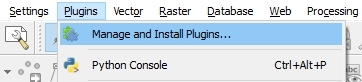
\includegraphics[width=200pt]{./pictures/manage_install.jpg}
      \caption{Open dialog of Plugins.}
      \label{fig:manage}
\end{figure}

\item{Go to \texttt{Settings} tab and press \texttt{Add...} button. Write
\url{http://geo.fsv.cvut.cz/geoforall/qgis-plugins.xml} to \texttt{URL}
and press \texttt{OK}. This way you add a path to plugin's home
repository CTU GeoForAll Lab because right now the plugin is not
registered in the official QGIS repository. At this time plugin is
distributed as experimental so if you want to see it you have to tick
the checkbox \texttt{Show\ also\ experimental\ plugins}.}

\begin{figure}[H]
    \centering
      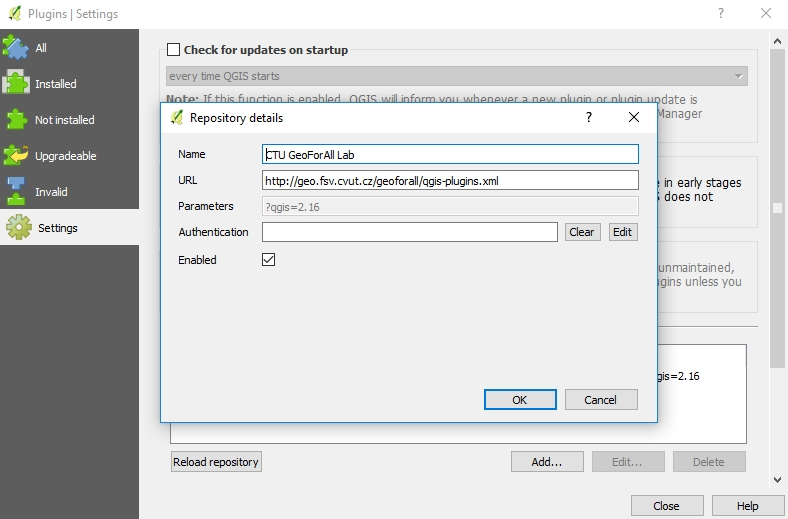
\includegraphics[width=400pt]{./pictures/home_repository.jpg}
      \caption{Add home plugin's repository.}
      \label{fig:repository}
\end{figure}

\item{Go to \texttt{All} or \texttt{Not\ installed} tab and search for
\texttt{Radiation\ \ Reconnaissance\ Results}. Select it and press
\texttt{Install\ plugin} button.}

\begin{figure}[H]
    \centering
      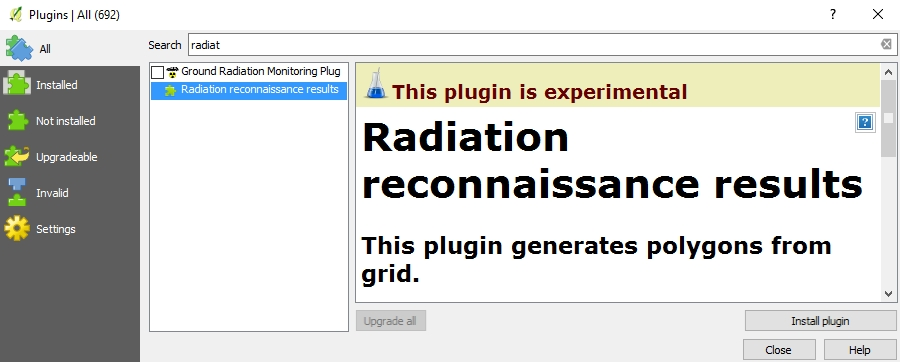
\includegraphics[width=300pt]{./pictures/install_search_plugin.jpg}
      \caption{Search and install the plugin.}
      \label{fig:install}
\end{figure}

\item{The Radiation Reconnaissance Results's icon is now shown in the QGIS
Plugins Toolbar and plugin is ready to use.}

\begin{figure}[H]
    \centering
      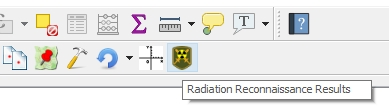
\includegraphics[width=200pt]{./pictures/toolbox.jpg}
      \caption{Radiation Reconnaissance Results Plugin on the QGIS toolbar.}
      \label{fig:toolbox}
\end{figure}

\end{enumerate}

\section{Plugin description}

\subsection{GUI}
\label{gui}
The plugin \zk{GUI} is divided into two tabs. The first of them is \texttt{Main}
tab:

\begin{figure}[H]
    \centering
      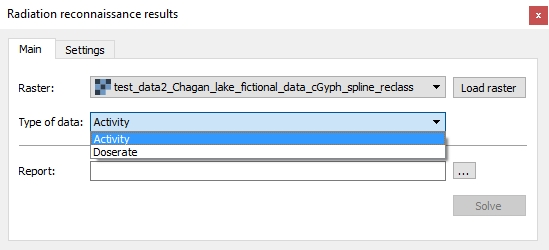
\includegraphics[width=300pt]{./pictures/main_tab.jpg}
      \caption{The main tab of plugin.}
      \label{fig:main}
\end{figure}

\begin{itemize}
\item{User selects the raster input and chooses appropriate input type (dose
  rate or surface activity). The raster combo box includes available
  layers from the Layer panel or it is possible to upload a raster file
  via button \texttt{Load raster}. By hitting this button, a file
  dialog opens and user can choose desired file (only \zk{GDAL} supported
  files are shown). Pressing \texttt{OK} will insert this path to the
  raster selection. Click on \texttt{Cancel} will interrupt the choosing
  dialog and the raster selection will not be changed.}
\item{Click on a tool button \texttt{...} opens a file dialog where user
  defines the path where the report file will be saved. This file is
  mandatory so \texttt{Solve} button is disabled until path is defined.}
\item{After pressing \texttt{Solve} button, plugin generates simplified
  polygons and saves output file(s) to selected destination(s).}
\end{itemize}

\newpage
The second tab of the plugin is \texttt{Settings} tab:

\begin{figure}[H]
    \centering
      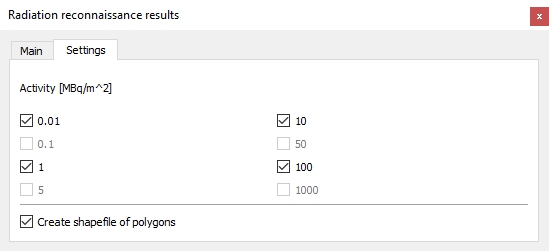
\includegraphics[width=300pt]{./pictures/settings_tab.jpg}
      \caption{The settings tab.}
      \label{fig:settings}
\end{figure}

\begin{itemize}
\item{This tab shows levels used for isolines generation. By default all
  levels available for selected input type are checked but user can
  uncheck particular ones.}
  	\begin{itemize}
		\item{For dose rates the preset levels are 0.1, 1, 5, 10, 50, 100 and 1000 cGy/h.}
		\item{For surface activities the preset levels are 0.01, 1, 10, 100 MBq/m2.}
	\end{itemize}
\item{The last check box allows user to decide if file of simplified
  polygons should be created. This output is optional but by default the
  check box is checked.}
\end{itemize}

\subsection{Input data}
\label{input-data}

\begin{figure}[H]
    \centering
      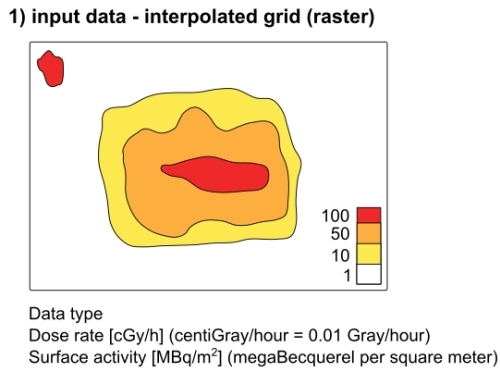
\includegraphics[width=250pt]{./pictures/input.jpg}
      \caption{Input file.}
      \label{fig:input}
\end{figure}

A raster grid of dose rate or surface activity with a format supported
by \href{http://www.gdal.org/formats_list.html}{GDAL library}. Dose rate
grid units has to be in cGy/h (centiGray/hour = 0.01 Gray/hour), surface
activities in MBq/m2 (megaBecquerel per square meter).

\subsection{Output data}
\label{output-data}

\begin{itemize}
\item{\textbf{Report (mandatory)} 

Structure of the output text report is following:

\texttt{/{[}VALUE{]}{[}UNIT{]}/MGRS:{[}COORDINATE{]}/MGRS:{[}COORDINATE{]}/MGRS:{[}COORDINATE{]}//}
  where:

  \begin{itemize}
  \item{\texttt{VALUE} = dose rate value or surface activity value; decimal separator
    is dot}
  \item{\texttt{UNIT} = used unit in XYH format; where X = C (centi), M (mili), U
    (micro); Y = G (gray), S (sievert); or BQM2 (becquerel per square
    meter)}
  \item{\texttt{COORDINATE} = coordinates in MGRS system, alphanumeric characters}
  \end{itemize}

  All text must be in capital letters. The report must begin with a
  slash, everything between two slashes is called a field. Field 1 can
  contain up to 12 characters. Field 2 can have up to 50 reps (maximum
  50 coordinates), and each field can contain up to 15 characters behind
  the MGRS identifier (eg. accuracy in meters). The last coordinate ends
  with a double slash (indicates the end of a line). Everything between
  the first slash and the double slash is called a line. Individual
  lines must be separated by line break. There must be no space before
  or behind the slash. There is no space between VALUE and UNIT. There
  is no space between \texttt{MGRS:} and the coordinate, the colon must be
  retained.

  The output may contain multiple rows, each being related to another
  level of the measured variable (eg, 3 rows sequentially for 1CGH,
  10CGH and 50CGH).}

\begin{figure}[H]
    \centering
      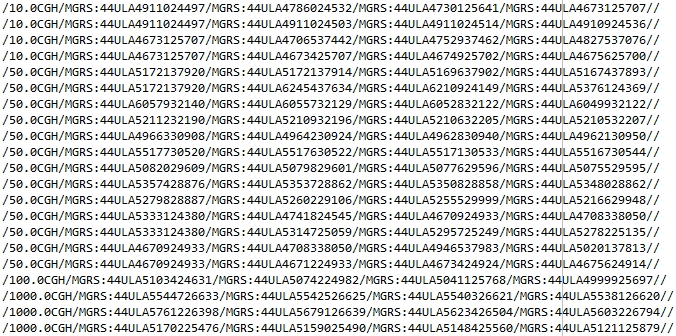
\includegraphics[width=375pt]{./pictures/vystupni_report.jpg}
      \caption{Output report.}
      \label{fig:report}
\end{figure}
      
\item{\textbf{File of simplified polygons} (optional)

  File of polygons in format Esri Shapefile (\textit{.shp}) is created if check
  box is checked. It is saved in the same directory as input raster
  file.}

\begin{figure}[H]
    \centering
      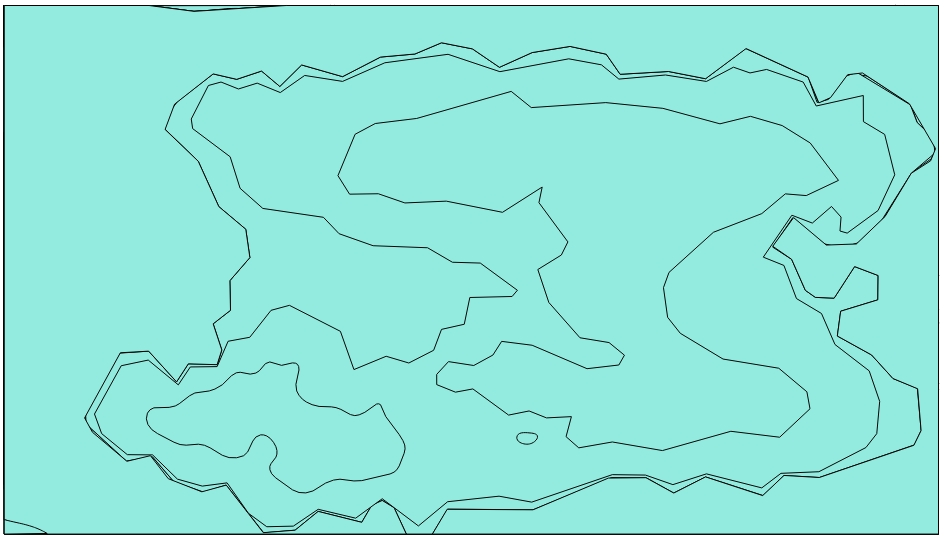
\includegraphics[width=350pt]{./pictures/vystupni_polygony.jpg}
      \caption{File of simplified polygons.}
      \label{fig:poly}
\end{figure}

\end{itemize}

\chapter{Obsah CD}
\label{cd}


\setlength{\unitlength}{.5mm}
\begin{picture}(250, 220)

  \put(  0, 212){\textbf{.}}

  \put(  1, 200){\line(0, 1){5}}
  \put(  1, 200){\line(1, 0){10} {\textbf{ src}}} 
  \put(150, 200){ zdrojový kód}  

  \put(  1,  190){\line(0, 1){10}}
  \put(  1,  190){\line(1, 0){10} {\textbf{ sample\_data}}}
  \put(150,  190){ testovací data}                     
          
  \put(  1,  180){\line(0, 1){10}}
  \put(  1,  180){\line(1, 0){10} {\textbf{ text}}}
  \put(150,  180){ text práce ve formátu PDF}
      
  \put(  1,  170){\line(0, 1){10}}
  \put(  1,  170){\line(1, 0){10} {\textbf{ zadani}}}
  \put(150,  170){ zadání bakalářské práce}
\end{picture}